\section{Nedre Grænser}%
\label{sec:nedregrænser}

\begin{frame}
  \frametitle{Pensum}
  \begin{itemize}
    \item Baase 2.4: \textbf{Informationsteoretiske nedre grænser for sortering ved sammenligninger}
    \item Jørgens noter: \textbf{Noter på nedre grænser}
    \item CLRS 9.3: \textbf{Median Problem}
    \item Weekly Note 11
    \item Video 22-24
  \end{itemize}
\end{frame}

\begin{frame}[allowframebreaks]
  \frametitle{Nedre grænser for sammenligningsbaseret algoritmer}
\begin{itemize}
  \item Et lower bound: $L(n)$ til et problem $P$ er et bevis for at \textbf{alle} algoritmer der løser $P$ bruger mindst $L$ operationer (e.g. sammenligninger)
  \item Her er $L(n)$ en løsning på input af størrelse $n$.
  \item Måden vi beviser på, er ved at bruge en ``adversary'', eller en modstander af en art.
  \item Målet med den her modstander, er at vedkommende \textbf{altid} vil vælge det værst mulige input for din algoritme.
  \item Dermed beviser man, at hvis en algoritme kan køre i en eller anden tid, e.g. $O(n \log n)$ på det værst mulige input, så har den en \textit{lower bound} på denne tid.
  \item Måden Jørgen stiller det op på, er ved at den her modstander faktisk \textit{genererer} modinputtet.
  \item Altså vil den næste sammenligning du laver gå til modstanderen, som så fortæller om inputtet er større end eller mindre end (eller lig med, som Jørgen siger ikke ændrer noget på argumentet hvis det er en mulighed.)
  \item \textbf{Eksempel}: Find et maksimum på en mængde af $n$ elementer.
  \item Ved en \textit{max} algoritme er det tydeligt at se at minimum er $n-1$, da alt under $n-1$ ville gå glip af mindst et af elementerne.
  \item En algoritme der kører på $n-1$ sammenligninger, vil kigge på hvert element lineært, og sammenligne med det tidligere største element.
  \item Det første element bliver ikke sammenlignet, men bliver sat til at være det største, og dermed er den ikke en del af de $n-1$ sammenligninger. Hvis den var havde det været $n$
sammenligninger.
  \item Et andet problem er at finde både maksimum og minimumselementet.
  \item Vi kan gøre dette på $2n-3$ sammenligninger:
  \item Først finder vi max på $n-1$ sammenligninger, og derefter min på $n-2$ sammenligninger.
  \item Vi fjerner elementet der var max i min-algoritmen, da vi ved at elementerne er distinkte.
  \item Dermed, ved at tage de to sammenligningstotaler sammen får vi $2n-3$.
  \item Vi kan dog gøre dette bedre. Vi kalder den følgende algoritme $A_{\min, \max}$, som laver $\frac{3}{2}n - 2$ sammenligninger.
  \item Vi skelner mellem om $n$ er lige eller ulige.
  \item Hvis $n = 2k, k \in \mathbb{N}$:
  \item Algoritmen vi kører laver par, og sammenligner dem. Parrene er med det første ulige element og det næste lige. Så altså $x_{1}$ og $x_{2}$ sammenlignes, og $x_{3}$ og $x_{4}$ etc, op til $x_{2k-1}$ og $x_{2k}$.
  \item I det tilfælde laver vi $k$ sammenligninger.
  \item Vi putter så alle elementerne i hver deres mængde. De mindste elementer i $S_{1}$ og de største i $S_{2}$.
  \item Dermed \textbf{ved} vi altså at min er i $S_{1}$ og max er i $S_{2}$.
  \item Det betyder også at $|S_{1}| = |S_{2}| = k$, da $n = 2k$.
  \item Vi kan så bruge hhv. den naive min algoritme og den naive maks algoritme til at finde min og maks i $k-1$ sammenligninger.
  \item Dermed bruger vi $k$ sammenligninger til at uddelegere til $S_{1}$ og $S_{2}$.
  \item Vi bruger $k-1$ sammenligninger til at finde min
  \item Vi bruger $k-1$ sammenligninger til at finde max
  \item I alt $k + k-1 + k-1 = 3k-2 = \frac{3}{2}n - 2$
  \item Hvad så hvis $n = 2k-1$ (altså hvis $n$ er ulige)?
  \item Vi vælger et element (det første, det sidste e.g.) til \textbf{ikke} at blive sammenlignet i et par.
  \item Når vi har kørt algoritmen som normalt, laver vi to ekstra sammenligninger: én for at tjekke om det udvalgte element er det største, og en for at tjekke om det er det mindste.
  \item Dermed $k-1$ sammenligninger for at finde $S_{1}, S_{2}$ (husk $n = 2k-1$)
  \item $k-2$ sammenligninger for at finde minimum
  \item $k-2$ sammenligninger for at finde maksimum
  \item $1$ eller $2$ sammenligninger for at finde om det udvalgte element er hhv. min eller max.
  \item I alt er antallet af sammenligninger $\le 3k-3 = 3(\frac{n+1}{2})-3 = \frac{3n}{2} - \frac{3}{2}$
  \item Vores mål er nu at vise at uanset hvor god en algoritme du har, vil du aldrig kunne komme under $\frac{3n}{2} - \frac{3}{2}$ sammenligninger.
  \item Lad $A$ være en arbitrær algoritmer der finder min og max, kun ved brug af sammenligninger. Lad $min$ være minimumselementet og $max$ maksimumselementet.
  \item Fra definitionen må $max$ være større end alle andre elementer, så $A$ \textbf{skal} bruge mindst $n-1$ stykker af information for at finde ud af om dette gælder.
  \item Vi bruger terminologien at ``vinde'' en sammenligning til at betyde at $x > y$, hvis $x$ vinder en sammenligning. På samme måde ``taber'' $x$ en sammenligning, hvis $x < y$.
  \item Dermed skal vi vide at $\max$ har \textbf{vundet} alle sammenligninger der kan laves.
  \item Den samme argumentation bruges for minimum.
  \item Nu stiller vi spørgsmålet: Hvor mange gange kan $A$ få 2 stykker af information på én sammenligning?
  \item Det eneste tidspunkt det er muligt på er hvis du sammenligner to elementer som både kunne have været maksimum og minimum. Altså hvis vi sammenligninger $x$ og $y$ betyder det at $x$ aldrig har vundet eller tabt en sammenligning, og $y$ har aldrig vundet eller tabt en sammenligning.
  \item Det vil altså sige at det er \textbf{højest} $\lfloor \frac{n}{2} \rfloor$ gange at dette kan ske.
  \item Måden vi viderbeviser på er ved at bruge grafer.
 \end{itemize}
 \begin{center}
 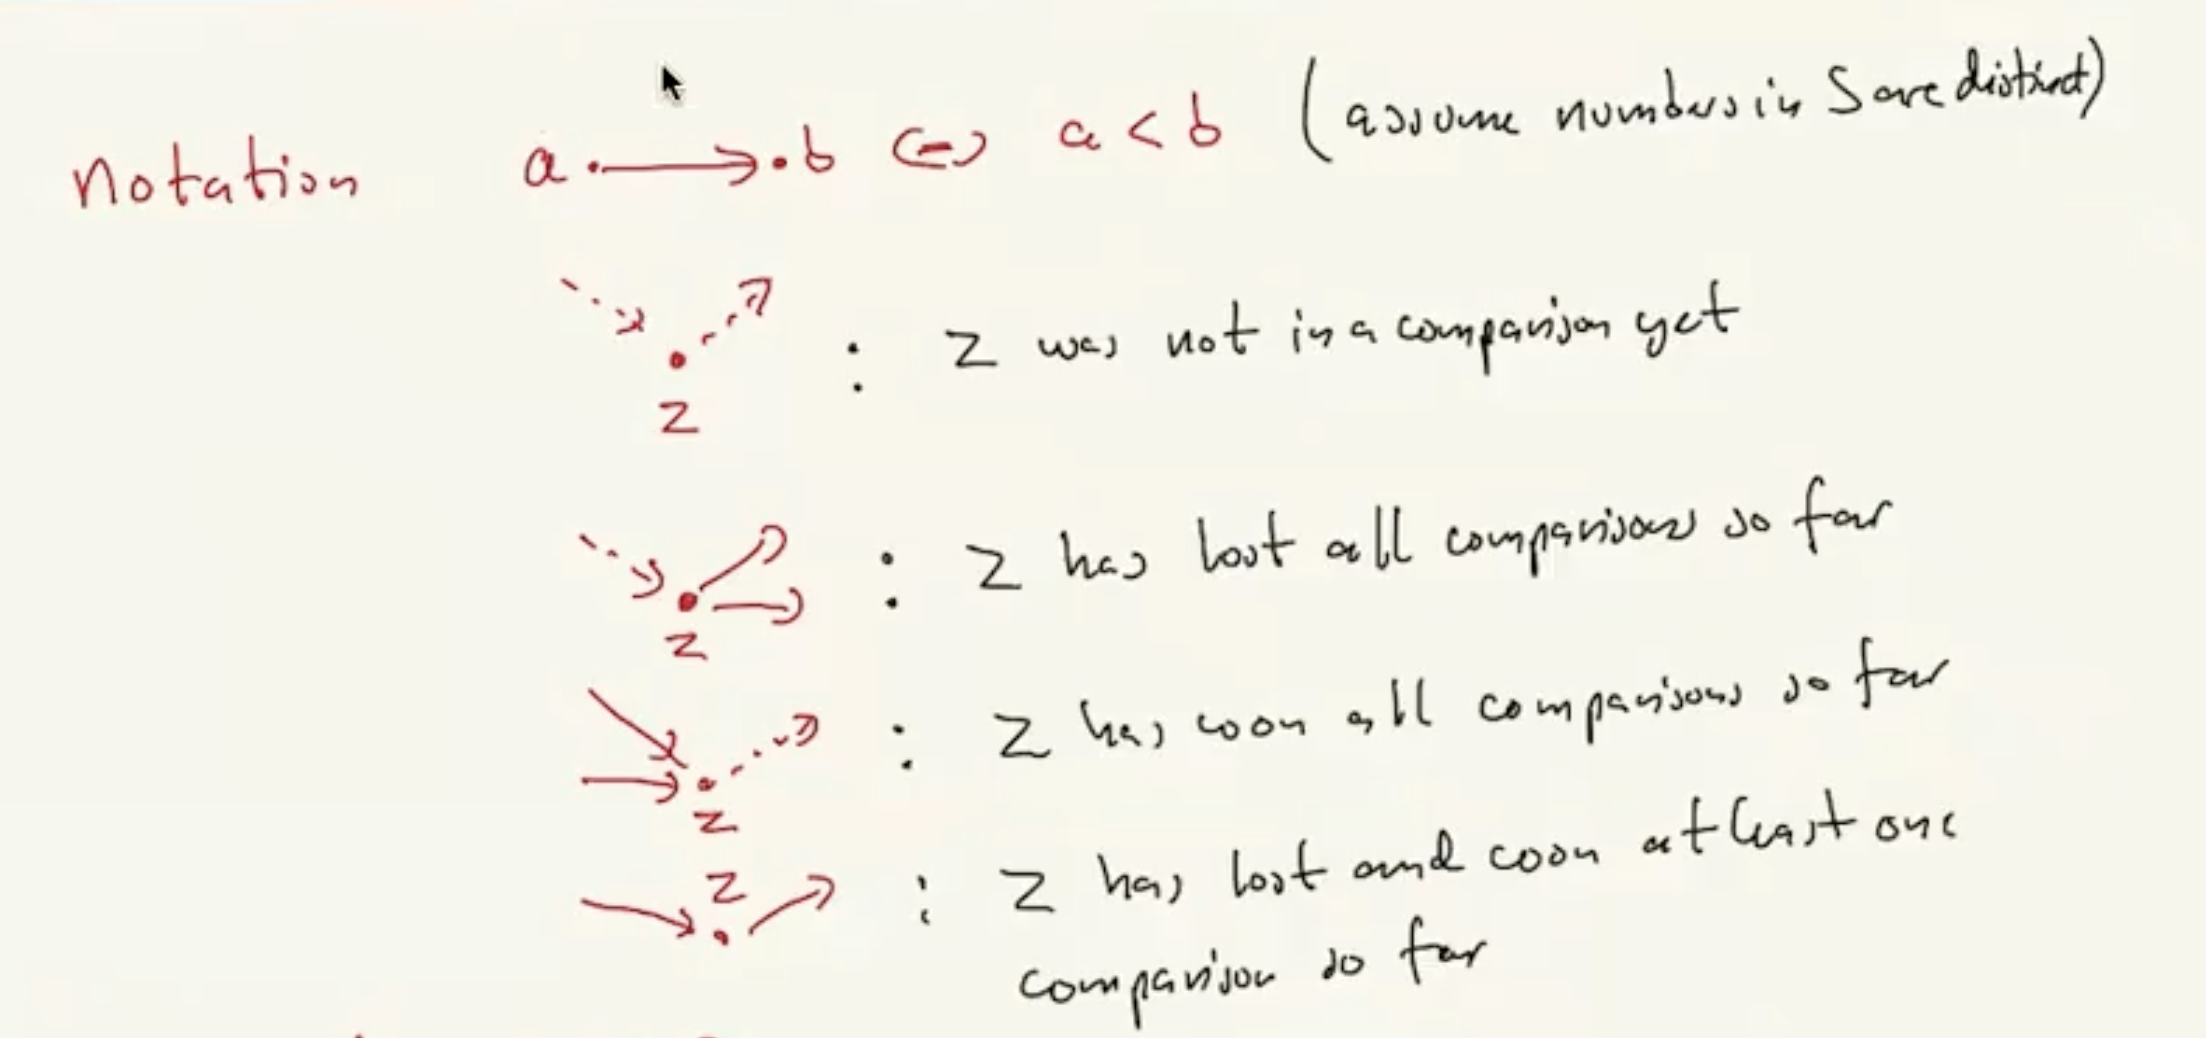
\includegraphics[scale=0.3]{figur/vid22a.png}
 \end{center}
 \begin{itemize}
   \item Her betyder de ``dashed'' pile, at der ikke er nogen pile, og normale pile at der er.
   \item Vi kommer nok til at bruge Jørgens noter en del her.
   \item Vi vil nu gerne vise hvordan modstanderen skal svare på spørgsmålet ``er $a < b$?''
   \item Måden modstanderen gør dette på, er ved at sikre at vi får så lidt information som muligt.
   \item Hvis $a$ aldrig er blevet sammenlignet med noget før og $b$ aldrig er blevet sammenlignet med noget før:
         \begin{itemize}
           \item Vi får 2 stykker information
           \item Modstanderen svarer $a < b$
         \end{itemize}
   \item Hvis $a$ aldrig er blevet sammenlignet med noget før, men $b$ har tabt alle sine sammenligninger:
         \begin{itemize}
           \item Vi får 1 stykke information
           \item Modstanderen svarer $b < a$
                 \begin{itemize}
                   \item Hvis modstanderen havde sagt $b > a$ kunne vi have vidst at $a$ ikke er maksimum, hvilket vi ikke ved nu.
                 \end{itemize}
         \end{itemize}

   \item Hvis $a$ aldrig er blevet sammenlignet før, og $b$ har enten vundet alle sine sammenligninger, eller både vundet og tabt.
         \begin{itemize}
           \item Vi får 1 stykke information
           \item Modstanderen svarer $a < b$
                 \begin{itemize}
                   \item Her finder vi ud af at $a$ ikke kan være maksimum, men ikke mere.
                 \end{itemize}
         \end{itemize}

   \item Hvis $a$ og $b$ har tabt alle sine sammenligninger:
         \begin{itemize}
           \item Vi får 1 stykke information
           \item Modstanderen svarer $a < b$
                 \begin{itemize}
                   \item Her får vi informationen at $b$ ikke kan være minimum
                 \end{itemize}
         \end{itemize}
   \item Hvis $a$ har tabt alle sine sammenligninger og $b$ har vundet alle sine:
         \begin{itemize}
           \item Vi får ingen information
           \item Modstanderen svarer $a < b$
                 \begin{itemize}
                   \item Der kommer ikke noget nyt af at sige det, hvilket er til gavn for modstanderen
                 \end{itemize}
         \end{itemize}

   \item Hvis $a$ har tabt alle sine sammenligninger, og $b$ har vundet eller tabt sine:
         \begin{itemize}
           \item Vi får ingen information.
           \item Modstanderen svarer $a < b$
                 \begin{itemize}
                   \item Her bliver vi bare ved den information at $a$ \textbf{kan} være minimum.
                   \item Hvis vi havde sagt det omvendt, ville vi vide at $a$ ikke kunne være minimum, og det samme kan $b$ heller ikke, da den har vundet.
                 \end{itemize}
         \end{itemize}
   \item De tre sidste argumenter, men omvendt (både $a$ og $b$ har vundet alle, etc.) gør vi bare det omvendte, altså modstanderen siger $b < a$
   \item Hvis $a$ og $b$ begge både har tabt og vundet, tjekker modstanderen om der er en vej fra $a$ til $b$, og hvis nej siger $a < b$, og ellers omvendt.
   \item Bemærk her, at som sagt før, er det kun i det første tilfælde vi kan få 2 stykker information.
   \item Det kan som sagt kun ske $\lfloor \frac{n}{2} \rfloor$ gange.
   \item Her bliver jeg lidt i tvivl. Jørgens \href{https://imada.sdu.dk/u/jbj/DM553/Slides21/Lect22.pdf}{slides} side 6.
   \item Jeg \textbf{tror} det der siges er at $\frac{n}{2} + n-2$ kommer fra at vi har delt det op, og så finder hhv. max og min i hver, liste, som vist tidligere.
   \item Nu stiller vi så spørgsmålet: Hvordan skal modstanderen svare når både $a$ og $b$ har tabt \textit{og} vundet mindst én  sammenligning?
   \item Modstanderen bruger ``acyclic orderings of partially ordered complete graphs''. Godt så.
   \item På dansk: acykliske ordninger af delvist ordnede komplette grafer
   \item Acyklisk = Ingen direkte kreds
   \item Acyklisk ordning = hvis $(u,v) \in E \Rightarrow i < j $. Dermed har \textbf{ikke alle} knuder en kant der går ud fra den. Hvis $\forall A \in V : D^{+}(A) \ge 1$, så er der en kreds.
   \item En turnering (tournament på engelsk) er en \textit{orientering} af en komplet graf.
   \item Så en turnering er altså, simpelt, bare en komplet graf, men med rettede kanter.
   \item Der findes kun én acyklisk turnering: nemlig hvor alle kanter gå fremad (hvis man antager en ordning $v_{1}, v_{2} \ldots v_{n}$).
   \item Hvis $D = (V,E)$ er en acyklisk graf og $n = |V|$, så kan vi tilføje en mængde af kanter $E'$ således at $D + A'$ er en transitiv turnering (komplet orienteret turnering) $TT_{n}$. (Se slides side 8 for visuelt)
   \item Her ser vi også grunden til valgene som modstanderen tog tidligere med om hvorvidt $a < b$ eller omvendt: målet for modstanderen er at få den acykliske graf til at være korrekt.
   \item Igen er jeg lidt i tvivl her, men jeg mener at Jørgen foreslår at modstanderen bare giver værdier efter den transitive turnerings ordning.
   \item Vi kigger nu på et andet problem: mindste og andet mindste værdi.
   \item Vi kan lave en naiv algoritme der fungerer præcis ligesom den naive max,min algoritme, men hvor vi kører min, og så min igen, men med den mindste værdi fjernet.
   \item Dette giver os $2n-3$ sammenligninger.
   \item En anden metode er ``turneringsmetoden'' (som sjovt nok har intet at gøre med de turneringer vi lige har set).
   \item Her der antager vi først at $\exists k : n = 2^{k}$.
   \item Så sammenligner vi alle par af tal, og ``går videre'' med de mindste.
   \item Dernæst sammenligner vi de mindste, og går videre med de mindste.
   \item $\vdots$
   \item Til sidst er der to tal der skal sammenlignes (fordi $n = 2^{k}$, Jørgen siger det sagtens kan generaliseres, men vil ikke uddybe), hvor det mindste af de to så er minimumsværdien.
   \item Altså bliver der lavet $\frac{n}{2} + \frac{n}{4} + \frac{n}{8} \cdots$ sammenligninger, indtil $\frac{n}{k} = 2$.
   \item \textbf{Efter} vi har fundet minimum, går vi op i den her turnering, og kigger på \textbf{alle} de tal, som har været større end det tal vi fandt ud af var minimum, da hver af disse tal kan være det andet mindste (selv det første tal som minimumstallet slog.)
   \item Der er $\log_{2}n$ kandidater til at være det andet mindste element.
   \item Vi bruger $n-1$ sammenligninger for at finde minimumsværdien (hvorfor?) og $\log_{2}n-1$ for at finde anden minimum.
   \item I alt $n+\log_{2}n-2$ sammenligninger.
 \end{itemize}
 % 18:30
\end{frame}

%%% Local Variables:
%%% mode: latex
%%% TeX-engine: xetex
%%% TeX-command-extra-options: "-shell-escape"
%%% TeX-master: "main"
%%% End:
